\chapter{Design}
\label{chap:design}
As the project has utilised an iterative approach with the Kanban methodology, the design has changed and been refined throughout the project. The design of the software will be broken down into 3 sections, namely the design of the web application and the design of the ACI and vCenter configuration.

\section{Web Application}
\label{design:web-application}
\subsection{Architecture}
\label{design:web-application:architecture}

A client-server architecture will be utilised to provide the user-facing experience, and the automation and data handling logic hosted on the server. By using this model, many clients can request and interact with data that is hosted on one central server. The backend and frontend that make up the application will be separate from one another, and will therefore be developed independently, with the frontend interacting with the backend via a REST API. This allows for the front end to be a SPA, which facilitates a better user experience due to the lack of page refreshes upon every request.

The server will process all requests generated by the front end and also make requests to the various APIs that will be required to automate the network deployment. The database will also store all data required by the server to generate the appropriate network configuration that is required to automate the deployment of projects to the network.

\begin{figure}[H]
    \centering
    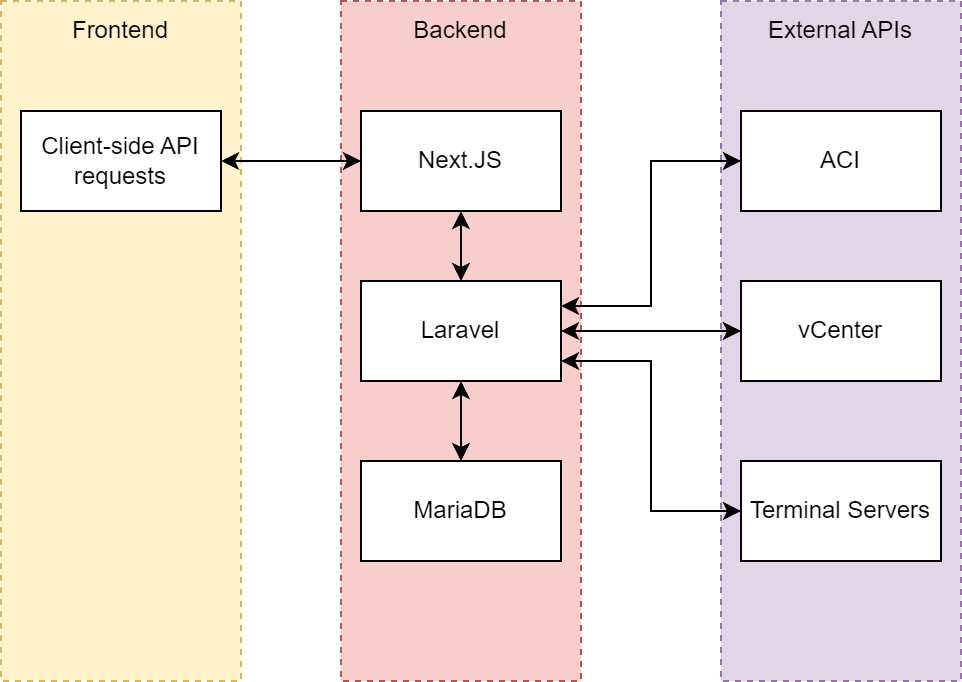
\includegraphics[scale=0.3]{images/web-architecture.png}
    \caption{Web Architecture Design}
    \label{fig:web-architecture}
\end{figure}

\subsection{Frontend}
\label{design:web-application:frontend}
Next.js will be used to power the frontend of the application as it is an enhancement of React.js and provides server-side rendering and acceleration of pages. React uses a modular 'componentised' approach to building the frontend, which allows for the creation of reusable components that can be used throughout the application. This allows for the creation of a modular and scalable frontend that can be easily extended and maintained.

React.js also has an extensive library of open-source components and libraries that can be utilised to make developing the frontend easier and more feature complete. Due to the complexity of some required features, such as having a drag-and-drop interface for the recreation of the lab space, the use of a library such as React Flow will be required as the time required to develop such a feature would be out of the scope of this project.

\subsection{Backend}
\label{design:web-application:backend}
The backend of the application will be written in PHP, using the Laravel PHP framework. Laravel is a popular PHP framework that will accelerate the development process, as it features an inbuilt \gls{orm}, \gls{api} routing system and an authentication system that can be implemented. Laravel utilises SQL-based databases, and as such MariaDB will be used as the database for the application. Laravel also features an in-built \gls{http} client which will be required to interact with the \gls{aci} and vCenter \gls{api}s which are all \gls{rest}-based.

Laravel follows the \gls{mvc} architecture, however as the frontend is a React \gls{spa}, Laravel will only be used to provide and consume the data via its \gls{rest} \gls{api}.


\subsection{Database Design}
\label{design:web-application:database}
As the project will need to store data persistently, ensuring that the database has an appropriately designed schema will ensure that the data is stored in a way that is easily accessible and can be queried efficiently. The design of the database was tweaked and refined throuhgout the development process, however the final \gls{erd} is shown below in Figure \ref{fig:database-erd}.

\begin{figure}[H]
    \centering
    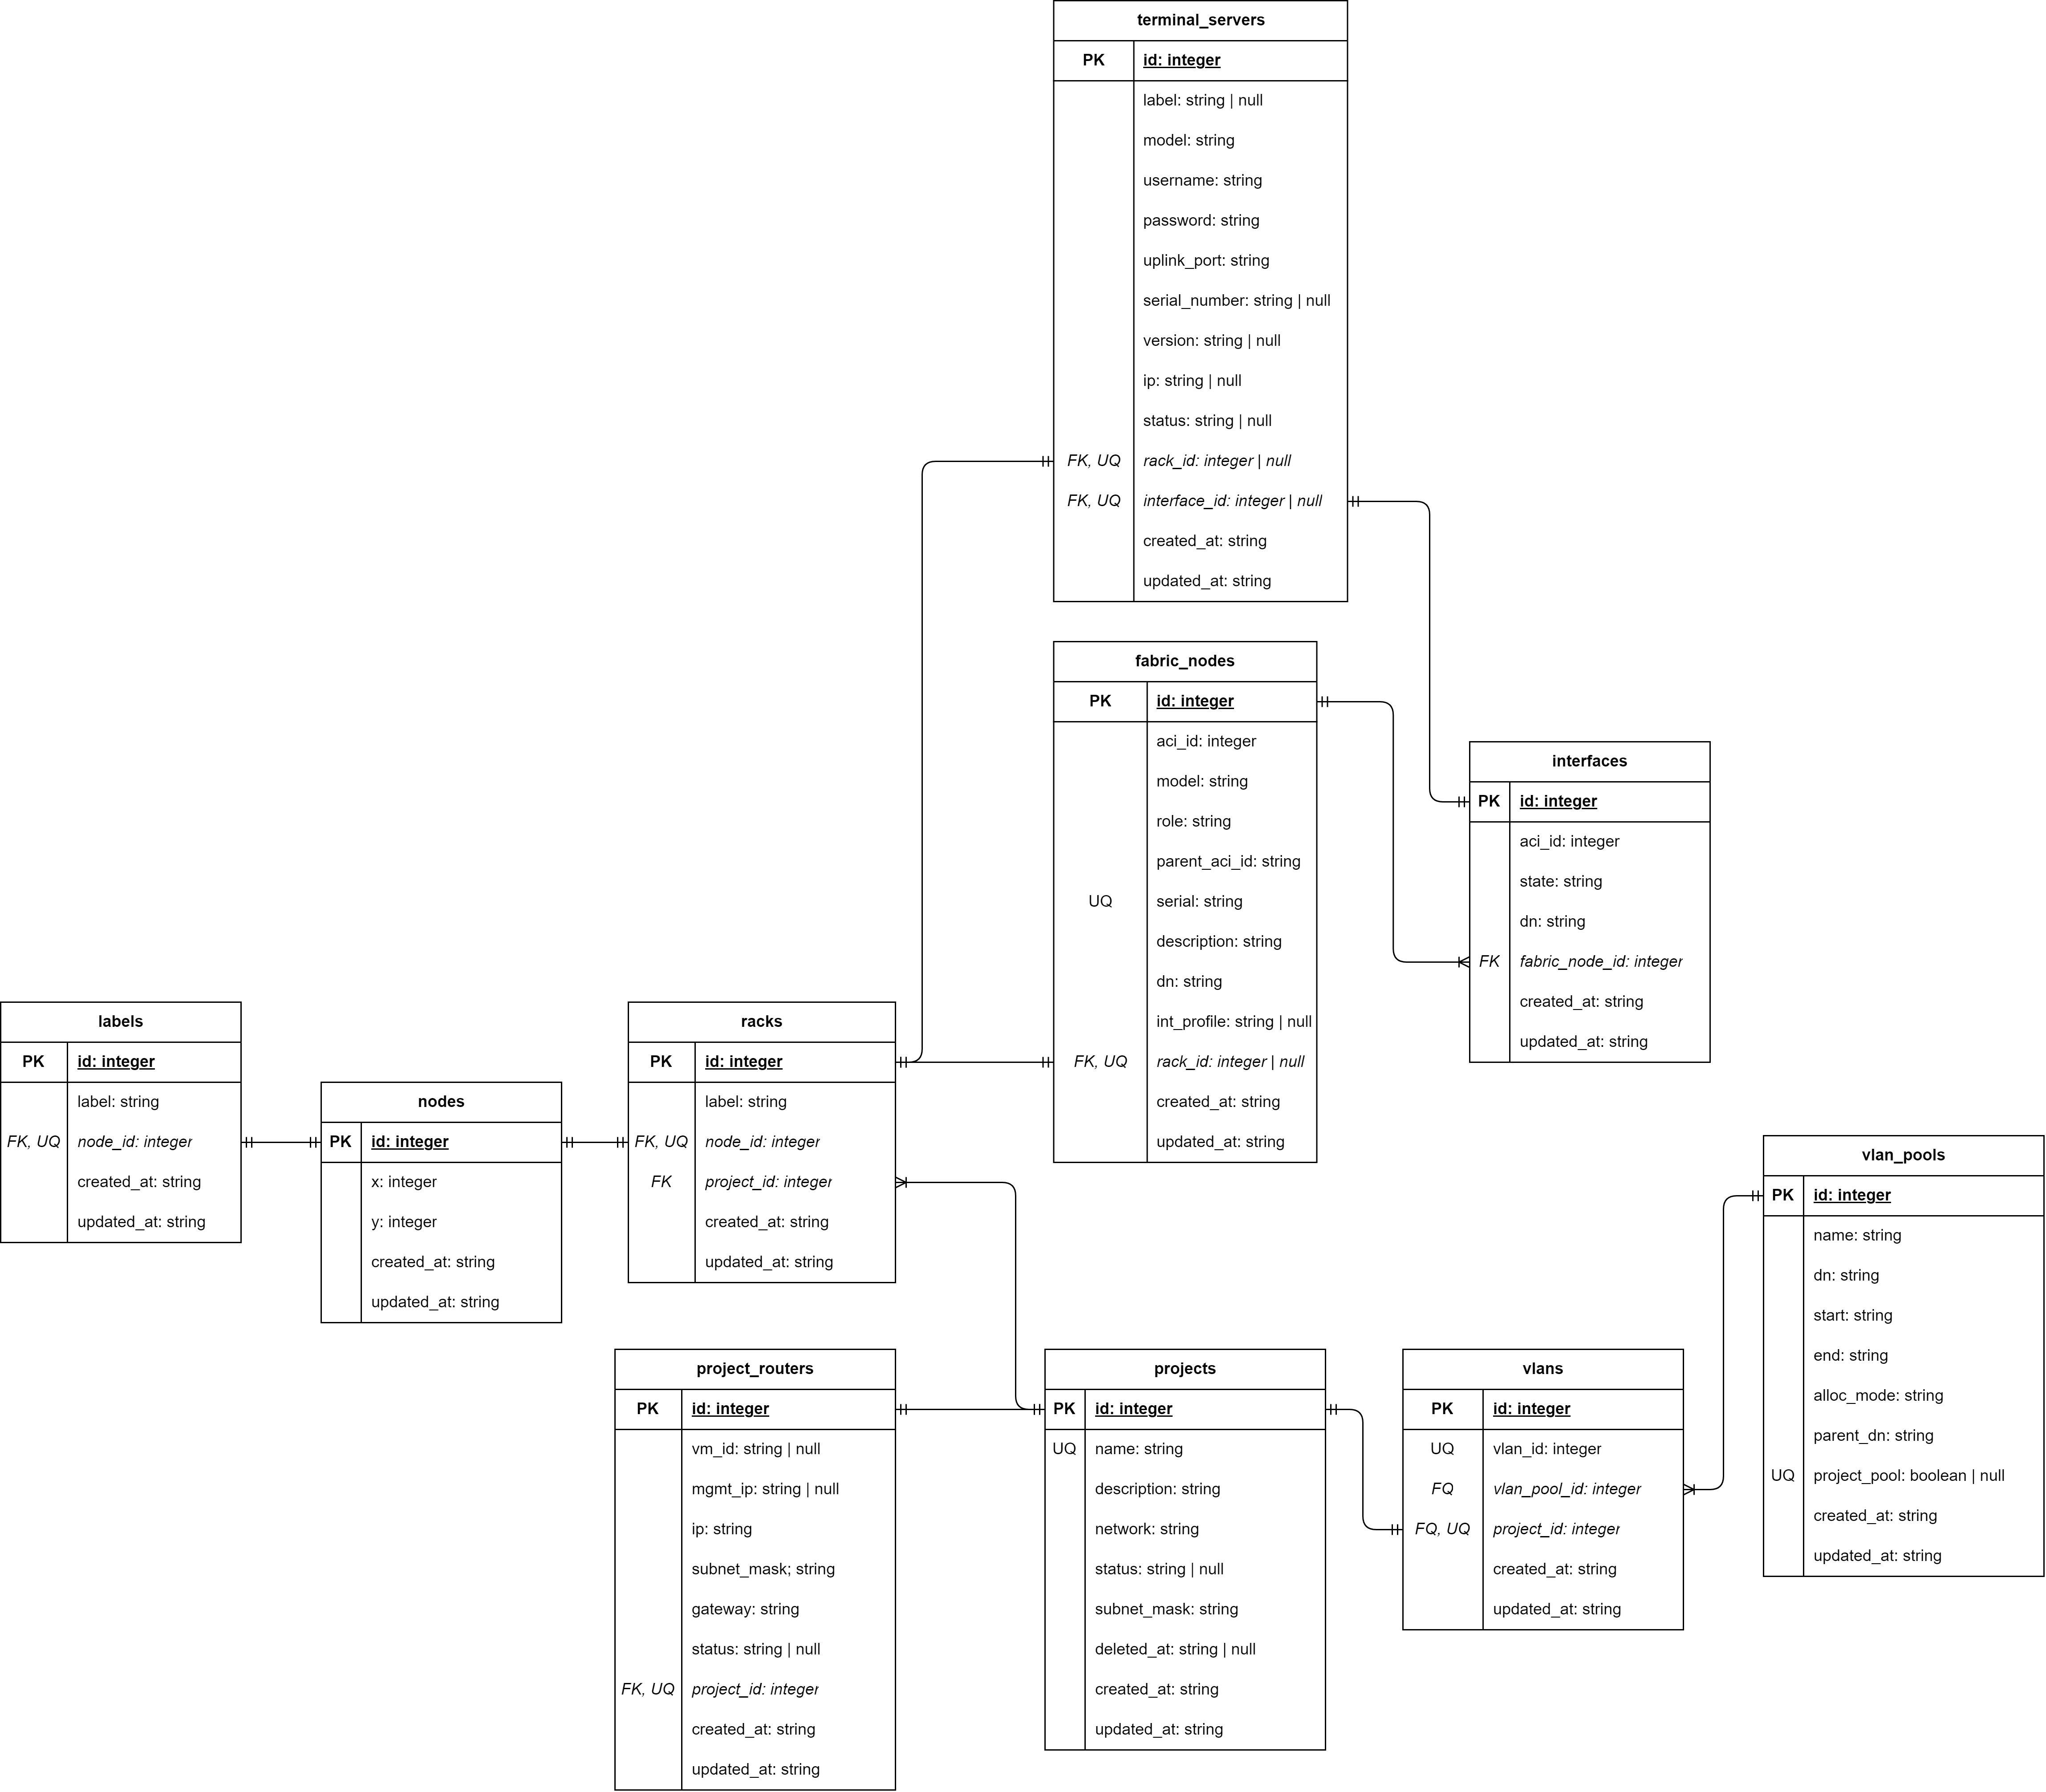
\includegraphics[scale=0.1]{images/erd.png}
    \caption{Database ERD}
    \label{fig:database-erd}
\end{figure}

\subsubsection{Nodes}
\label{design:web-application:database:nodes}
Nodes provide the root of storing information about the layout of the rackspace. Each node can either have a rack or a label attached to it. Labels will serve as a place to store text information on the rackspace diagram for informational purposes only. Racks will represent a physical rack in the rackspace. By using a node table, the position of the node can be abstracted away from the other data which is more relevant to the automation side. A more refined and efficient query is also possible as all nodes can be easily retrieved by selecting all nodes and then joining the rack and label tables to get the relevant information.

\subsubsection{Fabric Nodes and Interfaces}
\label{design:web-application:database:fabric-nodes-and-interfaces}
The fabric nodes and interfaces tables will be used to store information related to all fabric nodes that are attached to \gls{aci}. They will be automatically populated by the automation script which will retrieve information about the nodes and their associated interfaces from \gls{aci}. Each interface will tie to a fabric node so that all interfaces belonging to a fabric node can be easily retrieved. A role and parent ID field are also included in the fabric node table which allows for \gls{fex}s to also be stored as nodes. \gls{aci} treats \gls{fex}s as child nodes to leafs, hence why the parent ID and role field are needed to provide the correct differentiation between the two.

\subsubsection{Terminal Servers}
\label{design:web-application:database:terminal-servers}
The terminal servers table will store information about the various terminal servers present in the rack space, these will be inserted manually via the web UI. A relation will also exist that associates an interface to a terminal server so that the automation scripts can appropriately configure the uplink ports on the \gls{aci} fabric.

\subsubsection{Projects}
\label{design:web-application:database:projects}
The projects table will store all projects present in the application. Each project will link to the racks via a project ID field in the racks table. The project's private subnet will also be stored with the project.

\subsubsection{Project Routers}
\label{design:web-application:database:project-routers}
A project router will have a one to one relationship with a project, allowing only one project router per project. This table will keep track of the virutal router that is created for each project, and will also store the WAN IP address assigned to the router.

\subsubsection{VLANs and VLAN Pool}
\label{design:web-application:database:vlan-and-vlan-pool}
The VLAN pool table will store a list of all VLAN pools present in \gls{aci}. It will also store the selection that the user has made as to the VLAN pool that should be used by the automation platform for its endpoint groups. The VLANs table will be used to keep a record of which project is using which VLAN within a VLAN pool so that a VLAN cannot be used more than once.